\chapter{Results and analysis}

\section{Classification impovements}

Did classification improve, how, why

\begin{figure*}[htb]
  \centering
  \begin{subfigure}[b]{0.475\textwidth}
      \centering
      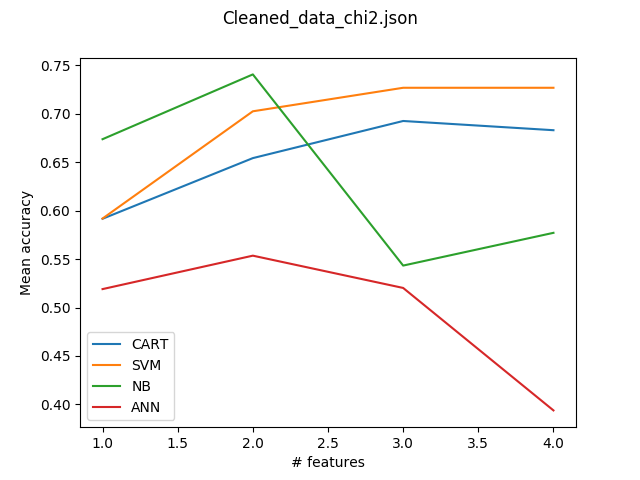
\includegraphics[width=\textwidth]{../plots_1d/Cleaned_data_chi2_combined.png}
      \caption[]%
      {{\small Dataset EN using Chi2}}
      \label{fig:EN_chi2}
  \end{subfigure}
  \hfill
  \begin{subfigure}[b]{0.475\textwidth}
      \centering
      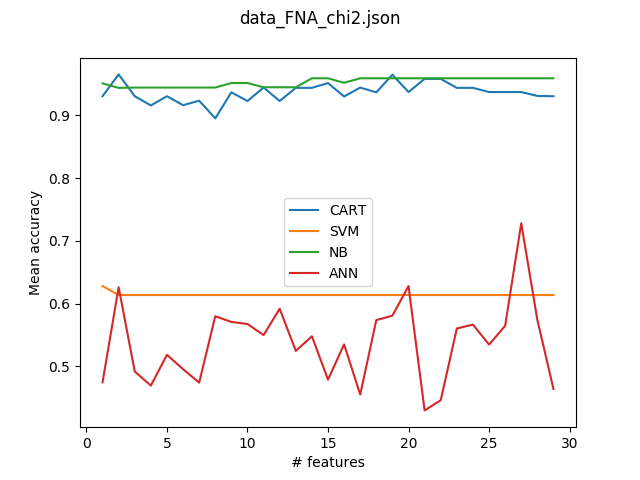
\includegraphics[width=\textwidth]{../plots_1d/data_FNA_chi2_combined.png}
      \caption[]%
      {{\small Dataset WBCD using Chi2}}
      \label{fig:WBCD_chi2}
  \end{subfigure}
  \vskip\baselineskip
  \begin{subfigure}[b]{0.475\textwidth}
      \centering
      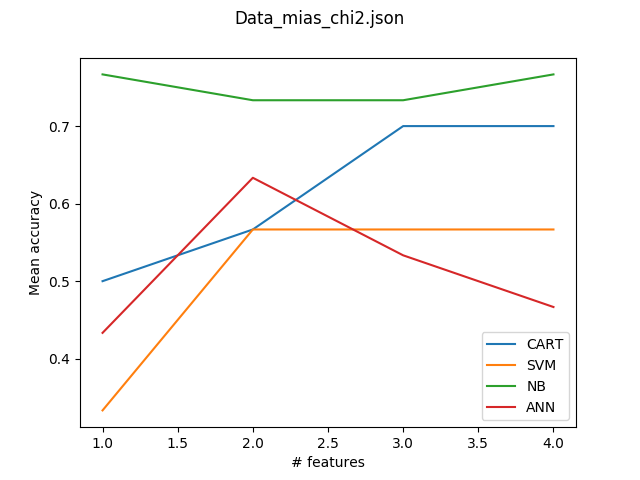
\includegraphics[width=\textwidth]{../plots_1d/Data_mias_chi2_combined.png}
      \caption[]%
      {{\small Dataset MIAS using Chi2}}
      \label{fig:MIAS_chi2}
  \end{subfigure}
  \quad
  \begin{subfigure}[b]{0.475\textwidth}
      \centering
      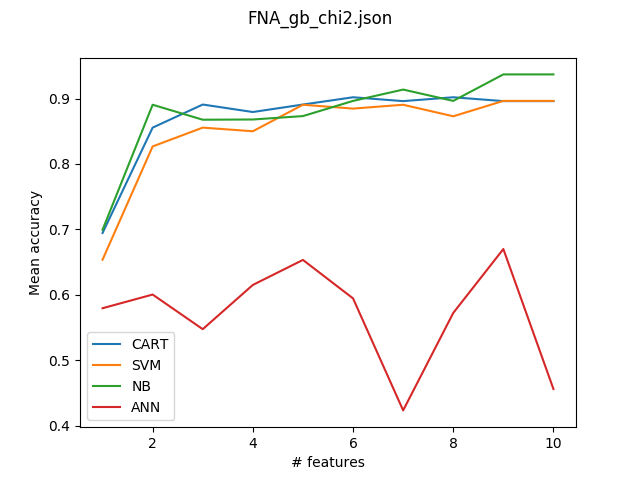
\includegraphics[width=\textwidth]{../plots_1d/FNA_gb_chi2_combined.png}
      \caption[]%
      {{\small Dataset RHH using Chi2}}
      \label{fig:RHH_chi2}
  \end{subfigure}

  \caption[ The average and standard deviation of critical parameters ]
  {Combined plots of all datasets comparing each classifier when using chi2 for feature selection.}
  \label{fig:plots_chi2}
\end{figure*}

\begin{figure*}[htb]
  \centering
  \begin{subfigure}[b]{0.475\textwidth}
      \centering
      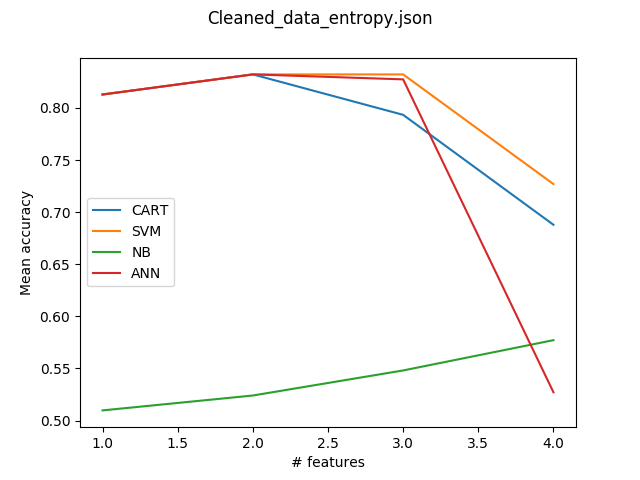
\includegraphics[width=\textwidth]{../plots_1d/Cleaned_data_entropy_combined.png}
      \caption[Network2]%
      {{\small Dataset EN using Entropy}}
      \label{fig:EN_entropy}
  \end{subfigure}
  \hfill
  \begin{subfigure}[b]{0.475\textwidth}
      \centering
      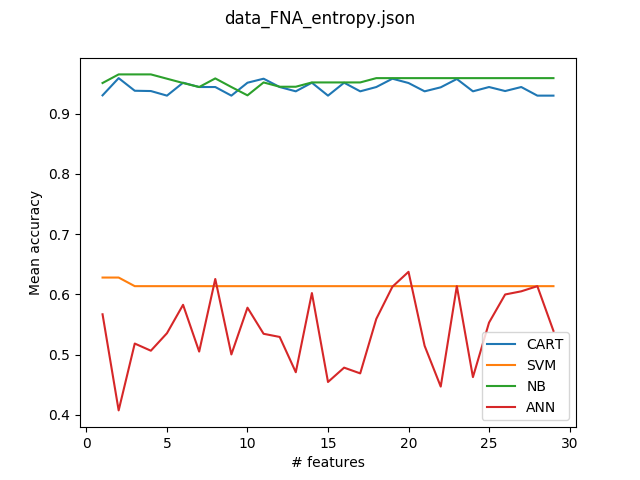
\includegraphics[width=\textwidth]{../plots_1d/data_FNA_entropy_combined.png}
      \caption[]%
      {{\small Dataset WBCD using Entropy}}
      \label{fig:WBCD_entropy}
  \end{subfigure}
  \vskip\baselineskip
  \begin{subfigure}[b]{0.475\textwidth}
      \centering
      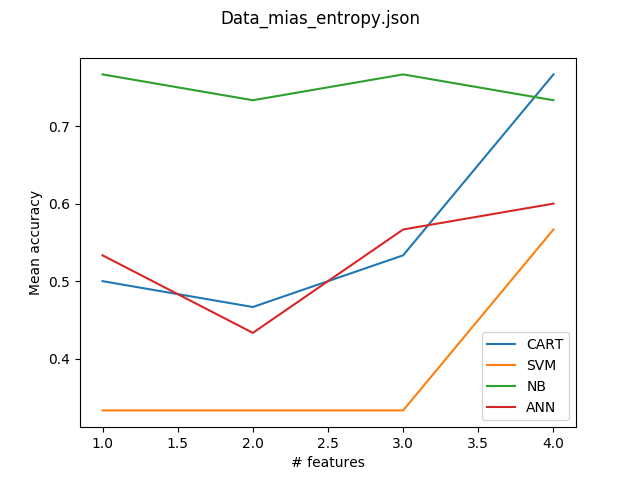
\includegraphics[width=\textwidth]{../plots_1d/Data_mias_entropy_combined.png}
      \caption[]%
      {{\small Dataset MIAS using Entropy}}
      \label{fig:MIAS_entropy}
  \end{subfigure}
  \quad
  \begin{subfigure}[b]{0.475\textwidth}
      \centering
      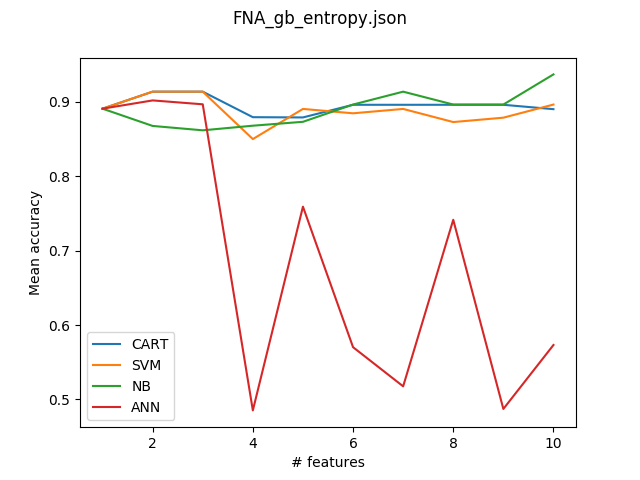
\includegraphics[width=\textwidth]{../plots_1d/FNA_gb_entropy_combined.png}
      \caption[]%
      {{\small Dataset RHH using Entropy}}
      \label{fig:RHH_entropy}
  \end{subfigure}
  \caption[]
  {{\small Combined plots of all datasets comparing each classifier when using Entropy for feature selection.}}
  \label{fig:plots_entropy}
\end{figure*}

\begin{figure*}[htb]
  \centering
  \begin{subfigure}[b]{0.475\textwidth}
      \centering
      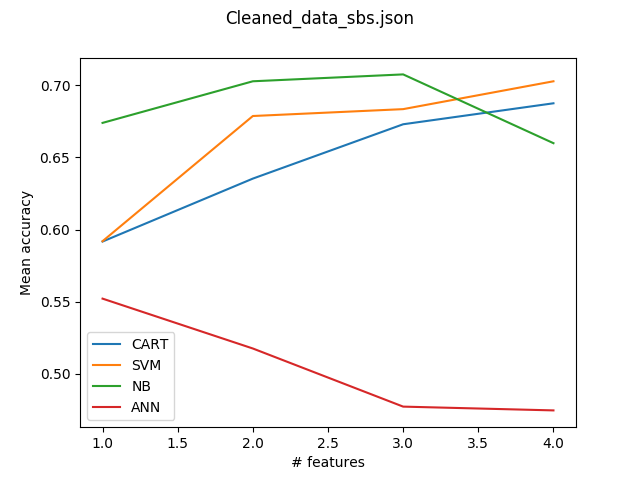
\includegraphics[width=\textwidth]{../plots_1d/Cleaned_data_sb_combined.png}
      \caption[]%
      {{\small Dataset EN using SBS}}
      \label{fig:EN_sbs}
  \end{subfigure}
  \hfill
  \begin{subfigure}[b]{0.475\textwidth}
      \centering
      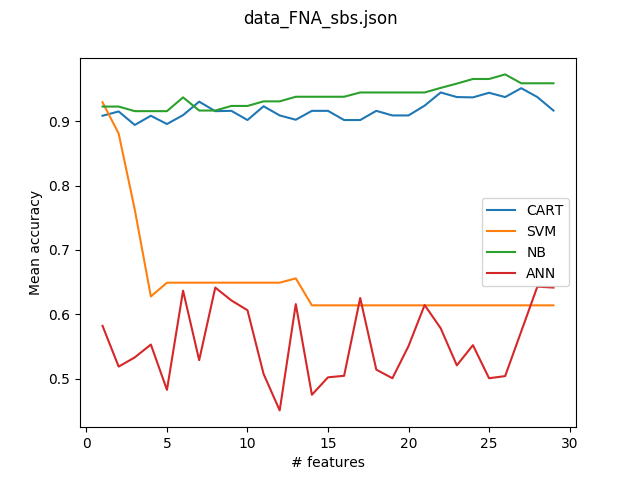
\includegraphics[width=\textwidth]{../plots_1d/data_FNA_sb_combined.png}
      \caption[]%
      {{\small Dataset WBCD using SBS}}
      \label{fig:WBCD_sbs}
  \end{subfigure}
  \vskip\baselineskip
  \begin{subfigure}[b]{0.475\textwidth}
      \centering
      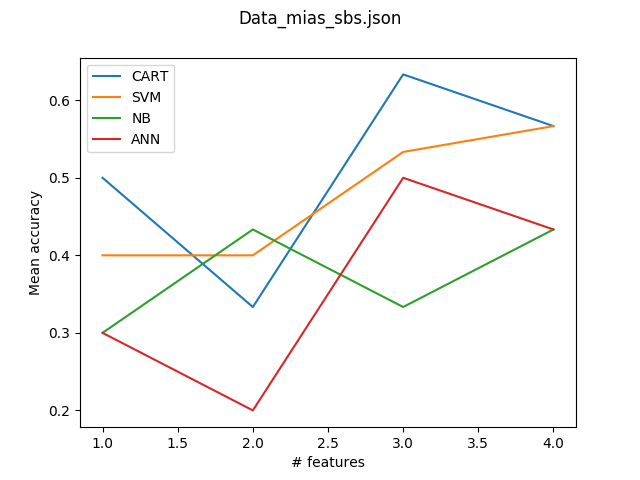
\includegraphics[width=\textwidth]{../plots_1d/Data_mias_sb_combined.png}
      \caption[]%
      {{\small Dataset MIAS using SBS}}
      \label{fig:MIAS_sbs}
  \end{subfigure}
  \quad
  \begin{subfigure}[b]{0.475\textwidth}
      \centering
      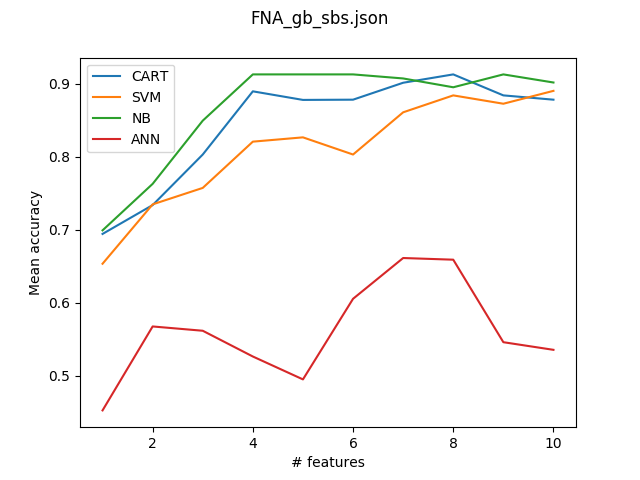
\includegraphics[width=\textwidth]{../plots_1d/FNA_gb_sb_combined.png}
      \caption[]%
      {{\small Dataset RHH using SBS}}
      \label{fig:RHH_sbs}
  \end{subfigure}
  \caption[]
  {{\small Combined plots of all datasets comparing each classifier when using SBS for feature selection.}}
  \label{fig:plots_sbs}
\end{figure*}

\begin{figure*}[htb]
  \centering
  \begin{subfigure}[b]{0.475\textwidth}
      \centering
      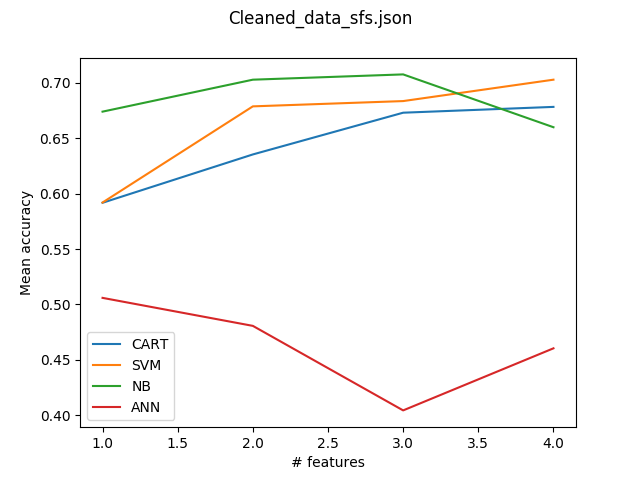
\includegraphics[width=\textwidth]{../plots_1d/Cleaned_data_sf_combined.png}
      \caption[]%
      {{\small Dataset EN using SFS}}
      \label{fig:EN_sfs}
  \end{subfigure}
  \hfill
  \begin{subfigure}[b]{0.475\textwidth}
      \centering
      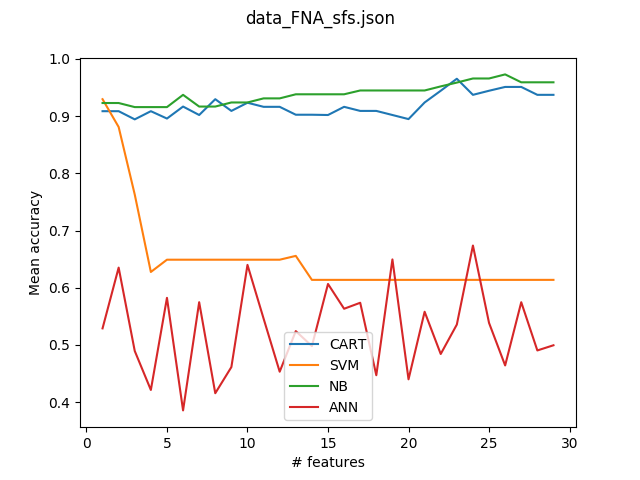
\includegraphics[width=\textwidth]{../plots_1d/data_FNA_sf_combined.png}
      \caption[]%
      {{\small Dataset WBCD using SFS}}
      \label{fig:WBCD_sfs}
  \end{subfigure}
  \vskip\baselineskip
  \begin{subfigure}[b]{0.475\textwidth}
      \centering
      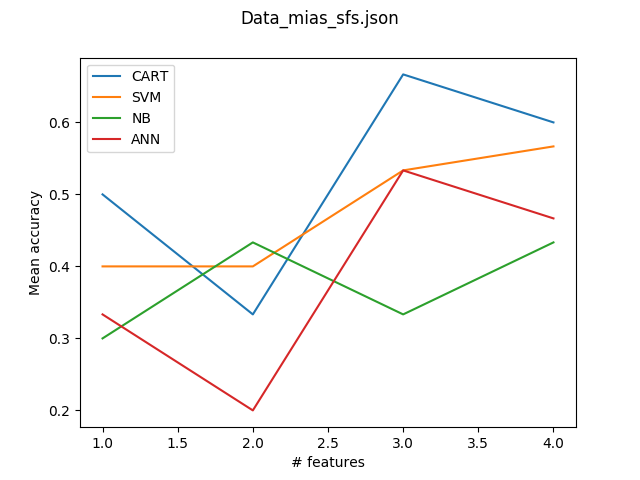
\includegraphics[width=\textwidth]{../plots_1d/Data_mias_sf_combined.png}
      \caption[]%
      {{\small Dataset MIAS using SFS}}
      \label{fig:MIAS_sfs}
  \end{subfigure}
  \quad
  \begin{subfigure}[b]{0.475\textwidth}
      \centering
      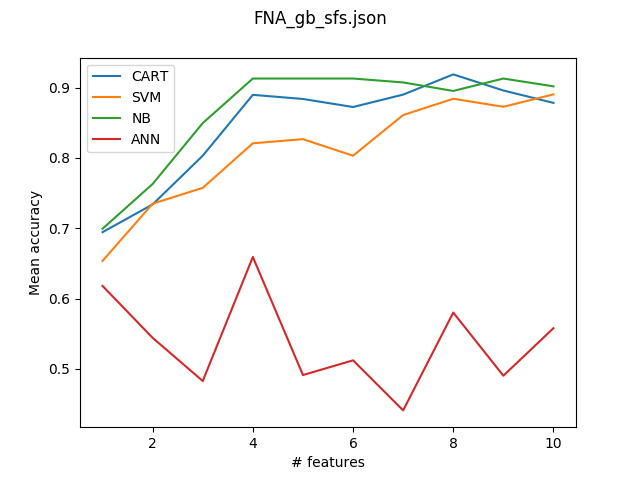
\includegraphics[width=\textwidth]{../plots_1d/FNA_gb_sf_combined.png}
      \caption[]%
      {{\small Dataset RHH using SFS}}
      \label{fig:RHH_sfs}
  \end{subfigure}
  \caption[]
  {{\small Combined plots of all datasets comparing each classifier when using SFS for feature selection.}}
  \label{fig:plots_sfs}
\end{figure*}

\begin{tabular}{|l|l|l|l|l|l|l|}
\toprule
{} & MIAS &   EN &  RHH & WBCD \\
\midrule
Chi2    & 0.58 & 0.59 & 0.64 & 0.71 \\
Entropy & 0.56 & 0.84 & 0.90 & 0.62 \\
SBS     & 0.54 & 0.55 & 0.59 & 0.74 \\
SFS     & 0.59 & 0.51 & 0.59 & 0.68 \\
Full    & 0.57 & 0.68 & 0.60 & 0.53 \\
Gain    & 0.04 & 0.24 & 0.51 & 0.41 \\
\bottomrule
\end{tabular}
 \\

\begin{tabular}{|l|l|l|l|l|}
\toprule
{} &    MIAS &      EN &     RHH &    WBCD \\
\midrule
Chi2    & 0.70000 & 0.69262 & 0.90196 & 0.96524 \\
Entropy & 0.53333 & 0.83214 & 0.91373 & 0.95905 \\
SBS     & 0.63333 & 0.67286 & 0.91307 & 0.95143 \\
SFS     & 0.66667 & 0.67286 & 0.91895 & 0.96524 \\
Full    & 0.76667 & 0.68786 & 0.89608 & 0.93714 \\
\bottomrule
\end{tabular}
 \\

\begin{tabular}{|l|l|l|l|l|}
\toprule
{} &    MIAS &      EN &     RHH &    WBCD \\
\midrule
Chi2    & 0.76667 & 0.74071 & 0.93693 & 0.95905 \\
Entropy & 0.76667 & 0.54810 & 0.91373 & 0.96524 \\
SBS     & 0.43333 & 0.70738 & 0.91307 & 0.97286 \\
SFS     & 0.43333 & 0.70738 & 0.91307 & 0.97286 \\
Full    & 0.76667 & 0.65976 & 0.93693 & 0.95905 \\
\bottomrule
\end{tabular}
 \\

\begin{tabular}{|l|l|l|l|l|l|l|}
\toprule
{} &    MIAS &      EN &     RHH &    WBCD & Row differences & Dataset diff \\
\midrule
Chi2    & 0.56667 & 0.72690 & 0.89641 & 0.62810 &         0.01429 &     -0.07500 \\
Entropy & 0.33333 & 0.83214 & 0.91373 & 0.62810 &        -0.09649 &      0.00452 \\
SBS     & 0.53333 & 0.68333 & 0.88431 & 0.92952 &         0.22672 &     -0.00172 \\
SFS     & 0.53333 & 0.68333 & 0.88431 & 0.92952 &         0.22672 &      0.16500 \\
Full    & 0.56667 & 0.72690 & 0.89641 & 0.61381 &         0.00000 &          nan \\
\bottomrule
\end{tabular}
 \\

\section{Best features}

Could we tell which features contributes most to correct classification, how, why those

\section{Source of errors}

What can have caused faulty results, can our results be trusted?
